% !TEX encoding = UTF-8 Unicode

\Chapter{Adatbázis kapcsolat}


\setlength{\parindent}{12.5mm}Az Oracle Database Express Edition adatkapcsolat szempontból két fő komponensből áll, az egyik a szerver, a másik a kliens. Ez egy hierarchiailag alárandelt kapcsolat, a kliens kapcsolódik a szerverhez, adatokat kér, amiket a szerver feldolgoz és - ha a kliens megfelelő jogosultsággal rendelkezik - kiszolgál. A megfelelő működéshez egy szervernek futnia kell, amihez kapcsolódhat(nak) a kliens(ek). A szerver és kliens települhet ugyan azon eszközre (sőt, egyszerre lehet telepítve 32 és 64 bites verzió is, ami több esetben javasolt is), valamint futásuk is történhet egy időben és egy számítógépen, így a kis infrastruktúrával és alacsony költségvetéssel rendelkező vállalkozásoknak is megfelelő megoldás lehet. A több klienst használó vállalatok pedig jellemzően egy külön erre dedikált szerverhez kapcsolódnak, és arra nem is kötelező az adatbázis kezelő szoftver telepítése, mert az Oracle beépített adminisztrációs felületéről (rendelkezik grafikus felhasználói felülettel és parancssorral is) a legtöbb szükséges teendőt el lehet végezni, ám a szervert érintő rendszerbeállítások kizárólag parancssoron keresztül érhetőek és vegezhetők el.

\Section{Kapcsolatok típusai}

\SubSection{Helyi kapcsolat}
	\label{helyi_kapcsolat}

Amennyiben a szerver és a kliens egy számítógépen fut, a kapcsolat típusa \textit{Helyi kapcsolat}, tehát a klienssel egy lokális kiszolgálóhoz kapcsolódunk. Ilyen esetekben - bár egy eszközön futnak - a kliens és a szerver logikailag elkülönül egymástól, viszont a hálózati címzés a helyi hálózaton át valósul meg, tehát az elérés történhet a 127.0.0.1 IP címen, vagy a localhost néven keresztül. Ez hasznos lehet több klienst használó vállalat esetén, ahol a kliens gépek a lerakatokban, vagy külső raktárokban találhatóak, de a központi raktárban vagy szerverszobában található fő szervergépről is elérhető és menedzselhető az adatbázis.\par
\setlength{\parindent}{12.5mm}Bizonyos esetekben fennálhat a vállalat kérése, hogy csak a helyi kapcsolatot használó számítógépről legyen elérhető a napló tábla, ami a beépített eszközzel is elérhető, de célszerű ilyenkor is az alkalmazást használni, a már megszokott kezelőfelület miatt. Ez néhány soros módosítás után könnyen megvalósítható, így a kliens és szervergépeken futó programok már külön instanciák.

\SubSection{Távoli kapcsolat}
	\label{tavoli_kapcsolat}

Távoli kapcsolat esetén a felhasználónak lehetősége van egy általa meghatározott kiszolgálóhoz kapcsolódni, ehhez szüksége van az adott szerver IP címére, portjára és a rajta futó adatbázis verziójának megnevezésére. Ennek formálisan is meg kell felelnie, de a szintaktikához segítséget nyújt a bejelentkező ablakon található információs ikon. Alkalmas kliens gépek esetén külső raktárakból történő hozzáférésre, valamint adott szerver elérésére bárhonnan, amennyiben a szerver és a kliens online, az átjáráshoz használt port nincs blokkolva a tűzfal által, továbbá a felhasználó rendelkezik érvényes hozzáféréssel az adatbázishoz.\par
\setlength{\parindent}{12.5mm}Amennyiben az előző pontban említett kérés fennáll a vállalat részéről, úgy a csak távoli kapcsolattal rendelkező instanciák jellemzően nem kapnak jogot arra, hogy a napló táblát lássák. A napló tábla egyébként is alacsony szinten védett, de így információhoz sem juthatnak azok, akiknek egyébként sem lenne hozzá jogosultságuk.
\vskip 0.5cm
A távoli kapcsolat kézi beállításához segítség a következő, \ref{miskolci_egyetem_kapcsolat} pontban.


\SubSection {Miskolci Egyetem}
	\label{miskolci_egyetem_kapcsolat}
Ez az opció a szoftver megjelenésének és működésének bemutatásához készült. Ebben az esetben a szoftver a Miskolci Egyetem Általános Informatikai Intézeti Tanszékén található Oracle szerveréhez kapcsolódik, ez a kapcsolat jellemzően a tanulmányi időszakokban érhető el, akkor megbízhatóan működik. Az alkalmazás, az információ- és adatátvitel, valamint a hozzá tartozó kapcsolat megfelelően tesztelhető rajta.
Az ehhez tartozó belépési adatok:\par

Mivel ez is egy távoli elérés (a külön listázás csak a kényelmesebb használat érdekében történt), ugyan ez az adatkapcsolat kipróbálható a \textit{Távoli} opció használatával is, a belépéshez szükséges adatok, valamint az egyetemi Oracle adatbázis szerver elérhetősége: 

\begin{center}
\begin{tabular}{rl}
Felhasználónév: & \textit{\textbf{duritt}}\\
Jelszó: & \textit{\textbf{t6716g}}\\
Cím: & \texttt{193.6.5.58:1521/XE}
\end{tabular}
\end{center}

\par

Az adatbázis, amelyhez a szoftver ezen a kapcsolatul keresztül kapcsolódik elérhető a Miskolci Egyetem által a tanulmányi időszakban biztosított szerver APEX felületén is, ahol grafikusan és parancsokkal is módosíthatjuk az adatbázis tartlmát, valamint lekérdezéseket, kimutatásokat, metaadatokat is lekérhetünk, emelett web-es alkalmazást is generálhatunk ezen keresztül. Ennek elérése:

%ezt ellenőrizni!
<<ellenorizni>>

\begin{center}
\begin{tabular}{rl}
Cím: & \texttt{193.6.5.58:8080/apex}\\
Munkaterület: & \textit{\textbf{duritt}}\\
Felhasználónév: & \textit{\textbf{admin}}\\
Jelszó: & \textit{\textbf{t6716g}}\\

\end{tabular}
\end{center}

\Section{Adatkapcsolat felépítése}
Az Oracle adatbázis-kapcsolat felépítésénél az elnevezések tetszés szerintiek lehetnek, de célszerűek a beszédes nevek, hogy közben, vagy esetleg a későbbiekben a kód a fejlesztő számára átlátható legyen \textit{(kivételt képeznek ezalól a nagy költségvetésű fejlesztést igénylő szoftverek, amelyeknél a cél a visszafejtés lehető legnehezebbé tétele)}, felépítés szerint:

\begin{itemize}

	\item \texttt{OracleConnection con;}
		\\Egy \texttt{OracleConnection} típusú objektum, ami valójában egy kapcsolatleíró string, mely az Oracle adatbázisokkal való kapcsolatot kezeli.

	\item \texttt{DataSet ds = new DataSet();}
		\\A \texttt{DataSet} példányosítása a lekérdezett adatok adattáblában történő tárolásához.
		\\Ez egy adatbázis a memóriában, amelynek szerepe, hogy az adattábla osztályban létrehozott objektumokat tárolja.

	\item \texttt{DataTable dt = new DataTable();}
		\\Az adattábla (\texttt{DataTable}) objektum \texttt{dt} példánya egy logikai táblát hoz létre a memóriában az adatbázis-szerverről áthozott adatok alapján.Amikor ez megtörténik, a program közvetlenül innen olvas majd, és a felhasználó által létrehozott módosítások is itt tárolódnak. Ennek tartalma lehet:
		\begin{itemize}
		\item \textit{Táblák:} Logikailag összetartozó értékek halmaza, elrendezése sorokban és oszlopokban történik.
		\item \textit{Mezők}: Cellák, melyekbe az adott cella típustáól függően adatot vihetünk be. Itt értékellenőrzés történik, azaz egy szám típusú cellába nem írhatunk karaktersorozatot.
		\item \textit{Sorok:} Jellemzően egy adott rekordhoz kapcsolódó értékek sorozata, a logikai szeparálást segítve külön cellákba rendezve, így a sorban lévő mezők alkoltnak oszlopokat.
		\item \textit{Oszlopok:} Az említett elrendezés függőlegesen összetartozó elemei, például telefonszámok egymás alatt. Létezhetnek oszlopok, amelyek elemeinek különbözőeknek kell lenniük, jellemzően ezek az elsődleges kucslok, egyedi azonosítók (ID).
		\item \textit{Nézetek:} Lekérdezés vagy több tábla kiválasztott oszlopai egymás mellett. Használatuk olyan esetekben történik, amikor több táblából szeretnénk adatokat egymás mellett úgy látni, hogy egy új nézőpontból közelíthessük meg a vizsgált tartalmat.
		\item \textit{Indexek:} A táblában lévő keresés felgyorsítására alkalmazott eszköz, jellemzően nagy méretű adatbázisokban használják, megvalósításai: hash-kód vagy bináris fa. Az optimalizálás és a megfelelően alkalmazott indexelés a nagy méretű adatbázisokban a futási időt $\mathcal{O}(n)$ -ről $\mathcal{O}(\log{}n)$-re csökkenti. Ez azt jelenti, hogy a nem megfelelően indexelt adatbázisok lineáris (az elemek számával egyenes arányban lévő) futási idejűek, tehát a az elemszámok növekedésével a futási idő is azonos mértékben nő, így ha az elemszám a duplájára nő, a futási idő is megduplázódik. A megfelelően indexelt adatbázisok esetén a futási idő logaritmikus, ami gyakorlatilag konstansnak vehető a logaritmus függvény miatt.
		\item\textit{ Kényszerek:} A kényszerek a táblákra és az abban szereplő oszlopokra vonatkozó, a megfelelő működés, konzisztencia biztosítását szolgáló szabályok. Több felhasználós környezetben a párhuzamos hozzáférés miatt problémás lehet, például ha egy időben szeretnének létrehozni megegyező azonosítójú terméket. Szintaktikailag a DDL része.
		\item \textit{Kapcsolatok:} Ahogy a relációs adatbázis elnevezés is utal rá, ezen adatbázis működésének alapja a táblák, mezők és értékeik közti kapcsolat, így ezeket is tárolni kell.
		\item \textit{Metaadatok:} Adatok az adatokról, amelyek a hatékonyság, integritásőrzés, adatvédelem biztosítását szolgálják.		
		\end{itemize}

	\item \texttt{OracleDataAdapter da = new OracleDataAdapter();}
		\\Ez az összekötő kapocs a fizikai adathalmaz és a memóriában tárolt, strukturált adathalmazok között.

	\item \texttt{OracleCommandBuilder builder = null;}
		\\Egy nem örökölhető osztály, amely automatikusan generálja azokat a parancsokat, amelyekkel a felhasználó által, futásidőben történő adatmódosításokat összeegyezteti a \texttt{DataSet}-ben lévő értékekkel.
	
	\item \texttt{OracleCommand cmd = new OracleCommand();}
		\\Az ehhez kapcsolódó átadott paraméterekkel (commandText (a lekérdezés szövege), \texttt{OracleConnection conString} (a kapcsolódást biztosító string)) egy új példányt hoz létre az \texttt{OracleCommand} osztályon belül, amellyel a lekérdezést majd végrehajtja.

	\item \texttt{string conString = String.Format("User Id=\{0\};Password=\{1\};" + "Data Source=\{2\};Pooling=false;", input\_uid, input\_pw, server\_address);}
		\\Ez a kapcsolódást biztosító string, azaz karaktersorozat.
		\\Jelen esetben egy formázott stringről van szó, mert az azonosító, jelszó és az adatforrás értékei a felhasználó általi input alapján kerülnek átadásra, de lehet előre definiált, statikus érték is. Erről bővebben a \ref{adatkapcsolat_parameterezese} szekcióban.

	\item \texttt{con = new OracleConnection(conString);}
		\\Ez az \texttt{Oracle} osztályon belül létező\textit{Connection} típus, ami az adatbázis eléréséért felel. Használatakor egy új példány jön létre az osztályban. Ez metódusként használható, így a zárójelben átadott \texttt{conString}-gel a kapcsolódáshoz szükséges adatok is átadásra kerülnek. Ennek értékei kerülnek átadásra a már létrehozott \texttt{con} változóba, és a későbbiekben ennek használatával jön létre a közvetlen adatkapcsolat.

	\item \texttt{con.Open();}
		\\Ha a példányosított \texttt{OracleConnection} megfelelő adatokkal rendelkezik, a \texttt{.Open()} metódus létrehozza a kapcsolatot a kliens és a szerver között. Amennyiben nincsenek megfelelő adatok, a metódus akkor is lefut, de a kapcsolódás sikertelen lesz.

\end{itemize}

\Section{Adatkapcsolat paraméterezése}
\label{adatkapcsolat_parameterezese}
A bejelentkező ablakon keresztüli bejelentkezéskor a kapcsolatot és az adatbázishoz való hozzáférés érvényességét maga az adatbázis-szerver ellenőrzi. A LoginFormba beírt felhasználónév és jelszó, valamint a manuális kapcsolódás esetén a kézzel beírt elérési cím (a helyinél és a távolinál is létezik cím, de ez a minidig ugyan az, így nem szükséges sem kézzel beírni, sem megjeleníteni) egy a kapcsolat felépítéséhez elengedhetetlen, a kapcsolódáshoz tartozó azonosítási és kapcsolódási adatokat tartalmazó stringbe (connectionString) kerül, így minidig a bejelentkező ablakba írt érték és a választott kapcsolat alapján, dinamikusan kap értéket.
\par
A paraméterátadás megvalósítása a forráskódban:

\begin{cpp}
string conString = String.Format(
		   "User Id={0};Password={1};" +
		   "Data Source={2};Pooling=false;",
		   input_uid, input_pw, server_address);
\end{cpp}

ahol:
\begin{itemize}
	\item{\itshape \{0\}} a felhasználónév (minden esetben a mezőbe írt érték adódik át),
	\item{\itshape \{1\}} a jelszó (minden esetben a mezőbe írt érték adódik át),
	\item{\itshape \{2\}} az adatkapcsolat címe (itt csak akkor adódik át a mezőbe írt érték, ha a listából a \textit{Távoli} van kiválasztva, egyébként választástól függően (\textit{Helyi} vagy \textit{Miskolci Egyetem}) előre definiált értékek adódnak át).
\end{itemize}

Ha az alkalmazást megrendelő fél nem szeretne a szoftverbe beléptető funkciót (ami nem javasolt, de a védelem megoldható különböző operációs rendszerbeli mechanizmusokkal, harmadik fél által készített szoftverekkel, vagy akár az eszköz teljes izolálásával, ugyanis a lokális szerveren futó adatbázishoz nem szükséges aktív internetkapcsolat), abban az esetben a connectionString felépítésének és tartalmának nem szükséges dinamikusnak lennie, statikus módon is megoldható:

\begin{cpp}
string conString = "User Id=Vallalat001;Password=Jelszo123;" +
                   "Data Source=127.0.0.1:1521/XE;Pooling=false;";
\end{cpp}

ahol:
\begin{itemize}
	\item a felhasználónév: \texttt{Vallalat001}
	\item a jelszó: \texttt{Jelszo123}
	\item az adatforrás: \texttt{127.0.0.1:1521/XE}, amiből:
	\begin{itemize}
		\item a szerver IP címe: \texttt{127.0.0.1}
		\item a port: \texttt{1521}
		\item az adatbázispéldány neve (SID): \texttt{XE}
	\end{itemize}
\end{itemize}



\begin{comment}

%innentol vecsie

\Section{Cartoon-style filter}

Az első filter egy rajzfilm jellegű (\textit{cartoon-style}) filter, amely az éleket kiemeli és a színeket elmossa. A szűrőhöz az ötletet Michael Beyeler hasonló szűrője adta, melyet Python nyelven készített el \cite{beyeler}.

A műveletekhez Gauss-piramist, kétoldalú szűrést, medián szűrést, illetve adaptív küszöbölést használtam. A szűrés eredményére egy példát \aref{fig:cartoon1}. ábrán láthatunk.

\begin{figure}[ht]
\centering
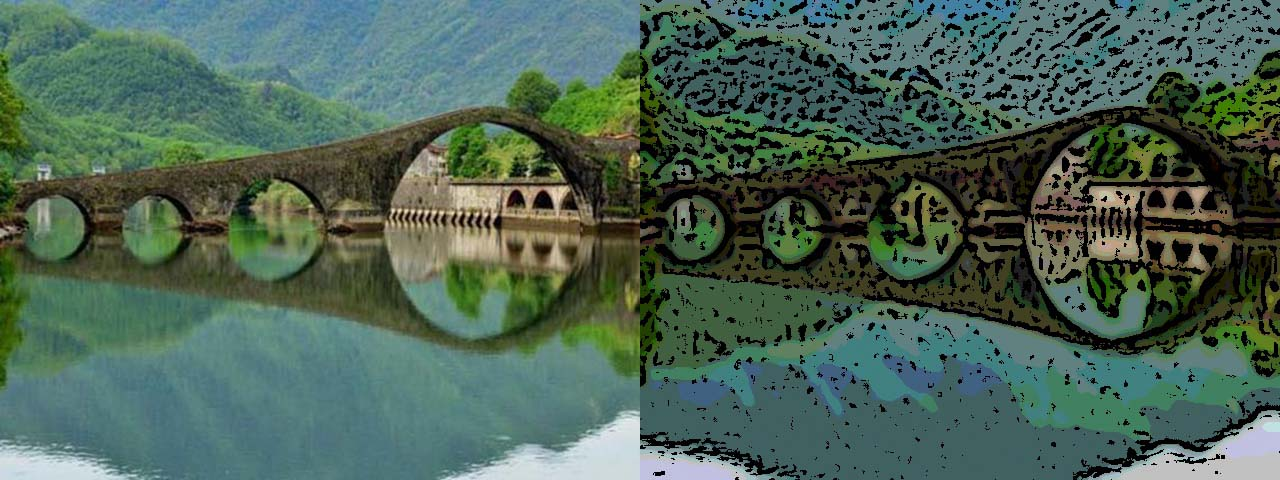
\epsfig{file=kepek/1_cartoon_filter.jpg, width=15cm, height=5.625cm}
\caption{Bal oldalon az eredeti-, jobb oldalon pedig a filterrel ellátott kép látható (forrás: \textit{http://www.erdekesvilag.hu/elkepeszto-tajkepek/})} 
\label{fig:cartoon1}
\end{figure}

\SubSection{Gauss-piramis és kétoldalú szűrő}

Első lépésben az eredeti képet lekicsinyítettem Gauss-piramis segítségével a kép méretének negyedére, rátettem egy kétoldalú szűrőt, majd vissza nagyítottam az eredeti méretre. A Gauss-piramis a kép kicsinyítése előtt Gauss-simítás segítségével súlyoz. A kétoldalú szűrő egy nem lineáris, élvédő és zajcsökkentő simító szűrő. Ezen lépés eredménye látható \aref{fig:cartoon2}. ábrán.

\begin{figure}[ht]
\centering
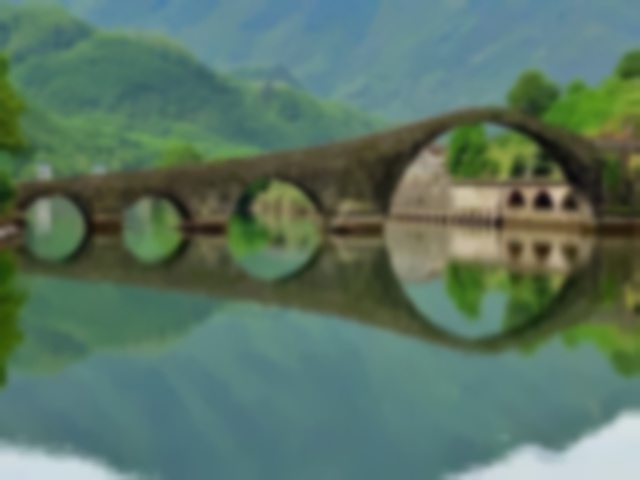
\epsfig{file=kepek/pyrambilateral.jpg,scale=0.5}
\caption{A Gauss-piramisban kicsinyítés és nagyítás valamint a kétoldalú szűrő eredménye } 
\label{fig:cartoon2}
\end{figure}

\SubSection{Színek konvertálása, medián szűrő}

Ebben a lépésben először az előzőleg kapott elmosott, színes képet átkonvertáltam szürkeárnyalatos képpé. 
Itt ki szeretnék térni magára a színes kép szürkeárnyalatossá konvertálására. Több féle megoldás létezik, ebből az elterjedtebbeket említeném. Az egyik az RGB komponensek átlagolása, de ez az emberi szem számára pontatlan, mivel nem egyformán érzékelünk minden színt. A következő lehetőség, amit az OpenCV- beépített színkonvertálása is használ az, hogy a komponensek súlyozott átlagát veszi, de nem egyenlő súlyértékekkel. Ennek a speciális esete, amely a HSV színrendszer \textit{value} értékét számítja. Ebben az esetben az OpenCV-s beépített kovertálást használtam a következő súlyokkal:
$$
\text{RGB to Gray} = 0.299 \cdot R+0.587 \cdot G + 0.114 \cdot B.
$$ 
Ennek eredményeként kapott képen medián szűrést hajtottam végre, amit ismét zajcsökkentés miatt alkalmaztam. Így a kép már teljesen el van mosva, egyre jobban rajzfilmszerű hatása van. Ennek az eredménye \aref{fig:cartoon3}. ábrán látható.

\begin{figure}[h!]
\centering
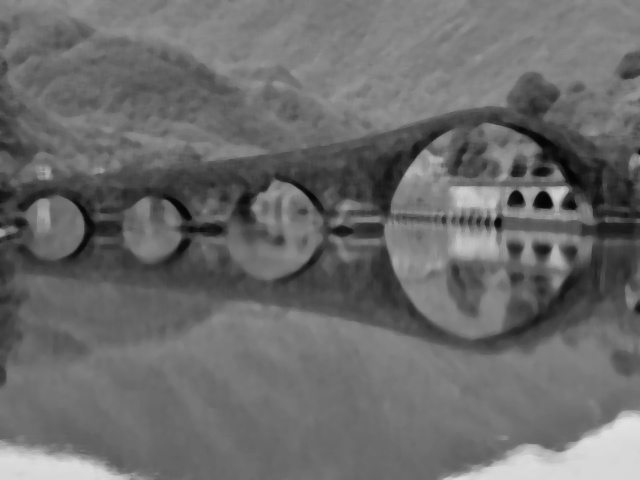
\epsfig{file=kepek/graymedian.jpg,scale=0.5}
\caption{Szürkére átalakított kép medián szűrővel} 
\label{fig:cartoon3}
\end{figure}

\newpage

\SubSection{Adaptív küszöbölés az élek kiemelésére}

Az adaptív küszöbérték általában szürkeárnyalatos vagy színes képet kap bemenetként, és a legegyszerűbb megvalósításban bináris képet eredményez. A kép minden egyes képpontjára egy küszöbértéket kell kiszámítani. Ez a küszöbérték lehet például egy kernelen belüli intenzitások átlaga, vagy egy, a hisztogram alapján becsült érték. Amennyiben a képpontérték a küszöbérték alatt van, akkor a háttérértékre van állítva, ellenkező esetben az előtérbe kerül.

\begin{figure}[h!]
\centering
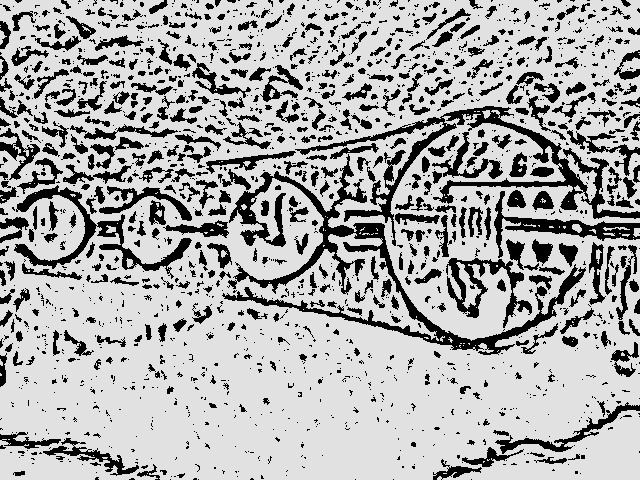
\epsfig{file=kepek/threshold.jpg,scale=0.5}
\caption{Az adaptív küszöbölés eredménye} 
\label{fig:cartoon4}
\end{figure}

\SubSection{A szűrőkkel és a küszöböléssel előállított képek egyesítése}

Az adaptív küszöböléssel elkészült maszkot át kell konvertálni színes képpé, hogy egyesíteni tudjuk az "elmosott" képpel amit az első két lépésben hoztunk létre. Ennek az elvégzését követően \aref{fig:cartoon5}. ábrán látható eredményt kaptuk.

\begin{figure}[h!]
\centering
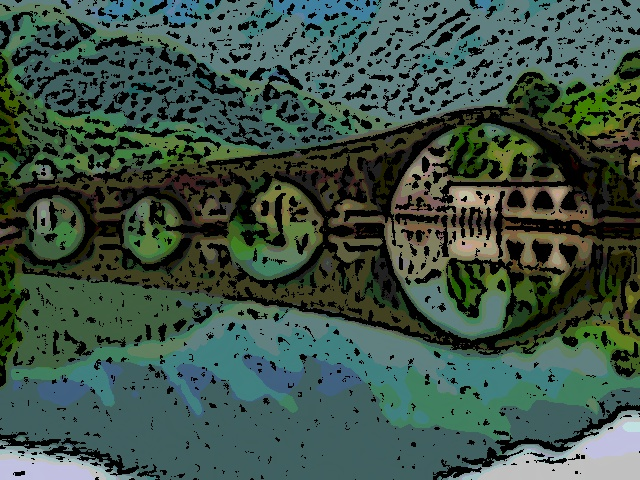
\epsfig{file=kepek/Cartoon_filter.jpg,scale=0.65}
\caption{Cartoon-style szűrő } 
\label{fig:cartoon5}
\end{figure}

% TODO: Esetleg pontszerű zajok eltávolítási módjáról lehet még néhány dolog a binarizált kép esetében.

\Section{Pencil sketch filter}

% https://github.com/MasteringOpenCV/code/blob/master/Chapter1_AndroidCartoonifier/Cartoonifier_Desktop/cartoon.cpp

Megpróbáltam egy olyan algoritmust létrehozni, ami egy ceruza rajzot imitál. A szakirodalomban találunk hasonló szűrési eljárásokat, mivel egy gyakran előforduló hatásról van szó \cite{beyeler2}.

A feldolgozáshoz szűrkeárnyalatosra konvertáltam a képet, medián szűrőt, Gauss szűrőt és egyéb képfeldolgozási műveleteket használtam, valamint egy "vásznat" is ráraktam, hogy még jobban olyan érzete legyen a képnek mint ha rajzolták volna (\ref{fig:pencil1}. ábra).

\begin{figure}[h!]
\centering
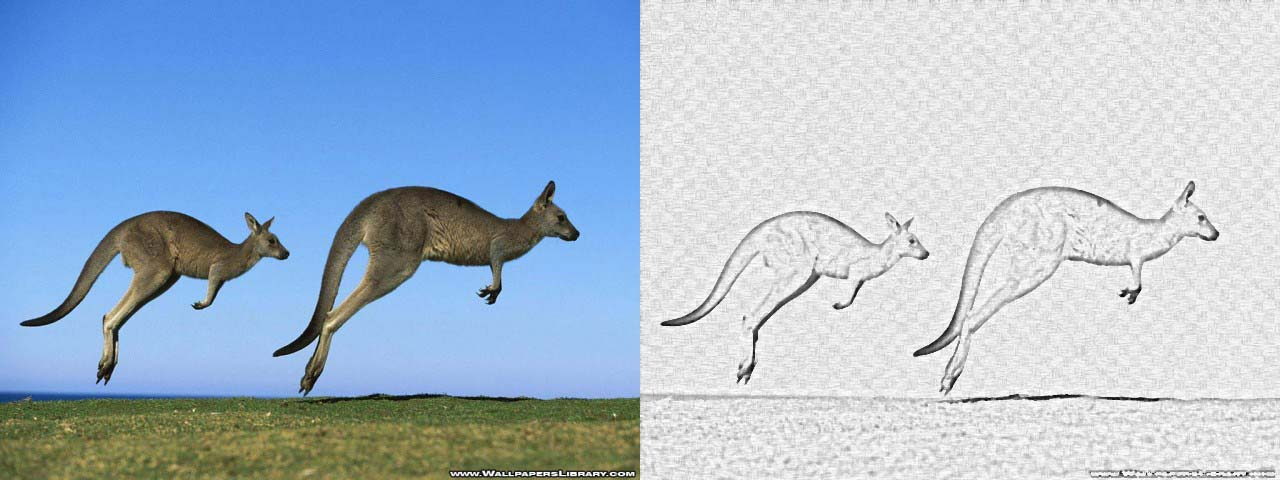
\epsfig{file=kepek/2_pencil_sketch_filter.jpg,width=15cm, height=5.625cm}
\caption{Bal oldalon az eredeti kép látható, jobb oldalon a filterrel ellátott kép $\quad$ (forrás: \textit{https://amazing.zone/kangaroos/they-only-can-go-forward})} 
\label{fig:pencil1}
\end{figure}

\newpage

\SubSection{Medián szűrő}

A kép szűrkeárnyalatos konvertálása után, végrehajtottam egy medián szűrést a kisebb, pont szerű zajok eltávolítása céljából (\ref{fig:pencil2}. ábra). A kernel méretétől függően már ez ad egy enyhe elmosást is a képhez, amely a végeredmény szempontjából előnyös.

\begin{figure}[h!]
\centering
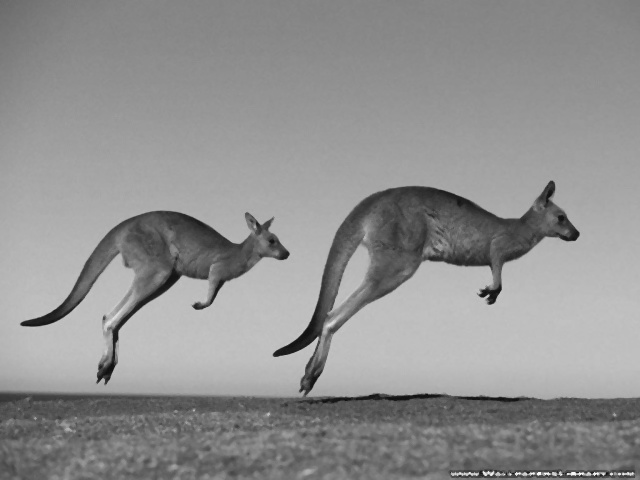
\epsfig{file=kepek/mediangray.jpg,scale=0.50}
\caption{Szürkére átalakított kép medián szűrővel} 
\label{fig:pencil2}
\end{figure}

\SubSection{Gauss szűrő}

Ezt a simítási teknikát, a képzaj  és a részletesség csökkentése érdekében használtam. Olyan sima elmosódást eredményez a képen, mint ha az nem lenne fókuszban (\ref{fig:pencil3}. ábra). A medián szűrőhöz képest lényeges különbség, hogy ezzel új árnyalatok is megjelennek a képen, a kontraszt összességében csökken.

\begin{figure}[h!]
\centering
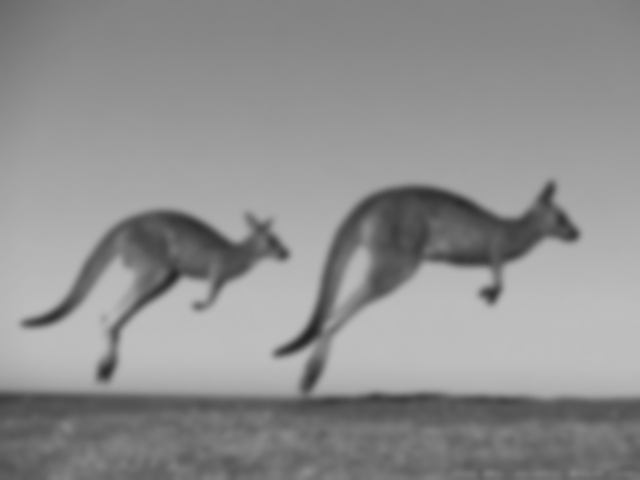
\epsfig{file=kepek/gauss.jpg,scale=0.5}
\caption{Gauss szűrő használata } 
\label{fig:pencil3}
\end{figure}

\SubSection{Az előző két lépés elosztása}

% TODO: Az osztást itt részletezni kicsit!

Az előző két szűrőt elosztottam egymással, így már tényleg majdnem olyan képet kaptam ami már ceruza rajz szerű. Úgy gondoltam még azért ráfér némi javítás, így még további műveleteket hajtottam végre rajta.

\begin{figure}[h!] 
\centering
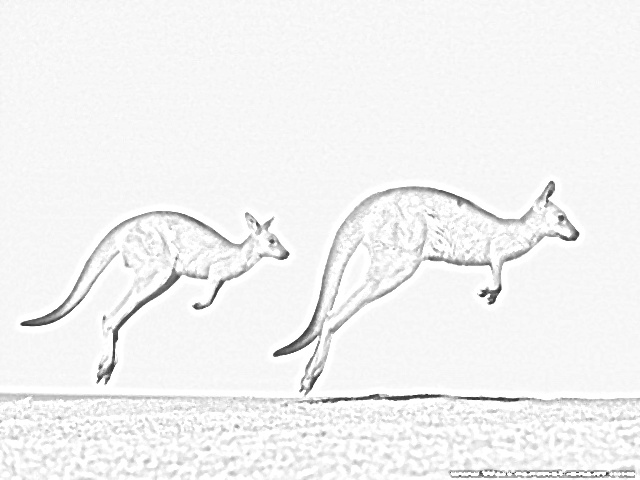
\epsfig{file=kepek/blend.jpg,scale=0.5}
\caption{Medián szűrés és a Gauss szűrés hányadosa } 
\label{fig: pencil4}
\end{figure}

\SubSection{Kontraszt széthúzása}

Azt figyeltem meg, hogy ha így hagyom a "Pencil sketch" szűrőt, akkor némely kép eléggé kontraszt szegény marad. Emiatt célszerűnek tünt belerakni egy kontraszt széthúzást, a szebb végeredmény érdekében. A széthúzás (vagy másnéven \textit{normalizáció}) egy egyszerű képjavító eljárás, amely megpróbálja javítani a kép kontrasztját azáltal, hogy "kiterjeszti" a benne lévő intenzitásértékek tartományát a kívánt értéktartományra. Ezt a műveletet követően a példaként szereplő képre \aref{fig:pencil5}. ábrán látható eredményt kaptam.

\begin{figure}[h!]
\centering
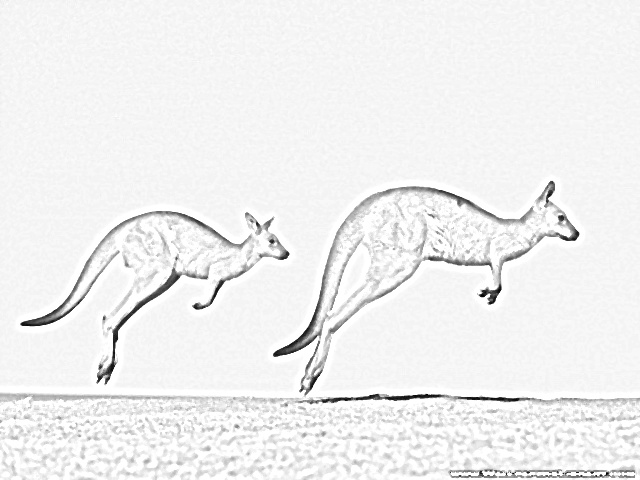
\epsfig{file=kepek/contraststrech.jpg,scale=0.5}
\caption{Kontraszt széthúzás} 
\label{fig:pencil5}
\end{figure}

\SubSection{Vászon hozzáadása}

A kontraszt széthúzása után, már egészen olyan hatása volt a képnek, mint ha egy ceruza rajz lenne. Ráraktam még egy "vászont" ami személyes véleményem szerint mégjobban segíti azt az érzetet hogy ez egy ceruzarajz. Először a vászonnak a színét át kellett konvertálnom színesből szűrkeárnyalatossá, hogy használható legyen a kontraszt széthúzott képhez (\ref{fig:pencil6}. ábra). Ezek után a vászont összeszoroztam az eddig eredményül kapott képpel, így jött létre a "Pencil sketch filter".

\begin{figure}[h!] 
\centering

\epsfig{file=kepek/canvasgray.jpg,scale=0.32}
\caption{Vászon színének konvertálása}
\label{fig:pencil6}
\end{figure}

\Aref{fig:pencil7}. ábrán láthatjuk a végeredményként kapott képet.

\begin{figure}[h!]
\centering
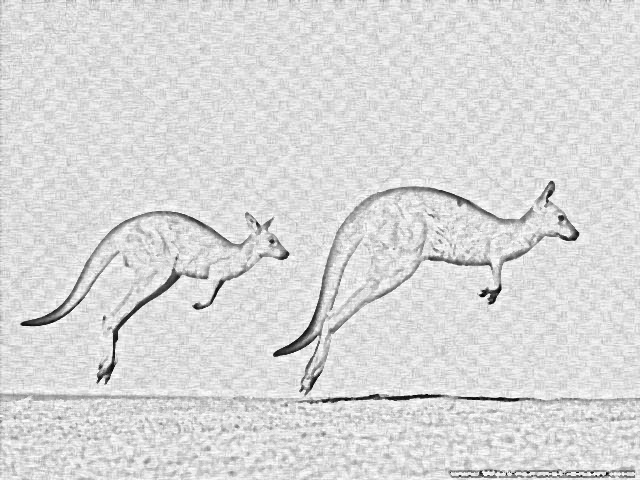
\epsfig{file=kepek/pencil_sketch.jpg, scale=0.4}
\caption{A \textit{Pencil sketch filter} eredménye} 
\label{fig:pencil7}
\end{figure}

\Section{Cartoon filter}

Megpróbáltam más technikával is létrehozni egy cartoon hatású képet, mivel a fellelhető irodalmakban is számos, különféle megoldást találni \cite{emami}.

Ahol medián szűrőt, Laplace éldetektálást valamit küszöbölést használtam (\ref{fig:2_cartoon1}. ábra).

\begin{figure}[h!]
\centering
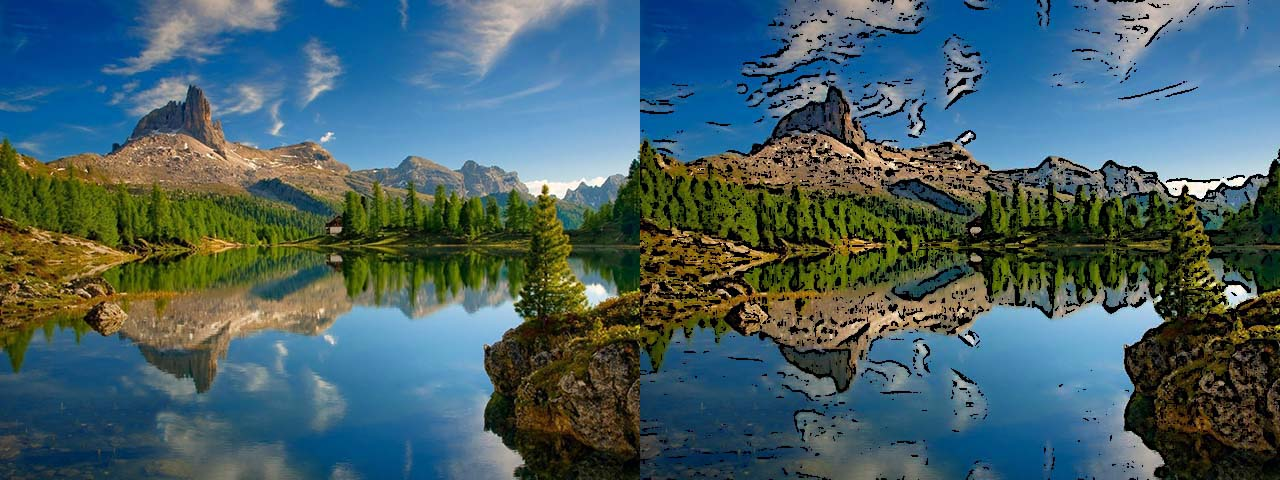
\epsfig{file=kepek/3_cartoon_filter2.jpg,width=15cm, height=5.625cm}
\caption{Bal oldalon az eredeti kép látható, jobb oldalon a filterrel ellátott kép $\quad$ (forrás: \textit{http://wallpaper-gallery.net/single/wallpaper-full-hd-nature/wallpaper-full-hd-nature-1.html})} 
\label{fig:2_cartoon1}
\end{figure}

\SubSection{Medián szűrő}

Mint az eddigi saját filtereknél, itt is előfeldolgozásként elvégeztem szürkeárnyalatossá konvertálást valamint egy medián szűrést (\ref{fig:2_cartoon2}. ábra).

\begin{figure}[h!]
\centering
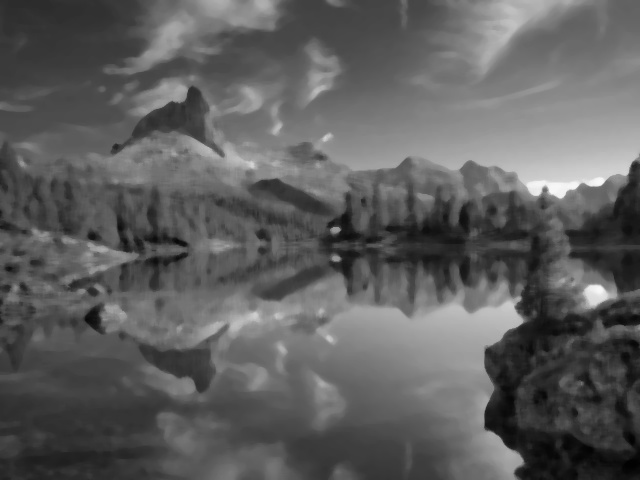
\epsfig{file=kepek/Cartoon1_gray.jpg,scale=0.45}
\caption{Szürkére átalakított kép medián szűrővel} 
\label{fig:2_cartoon2}
\end{figure}

\SubSection{Laplace éldetektálás}

Ennél a filternél a Laplace éldetektálást választottam. Ezzel olyan élmaszkot tudtam készíteni, amely kicsit hasonló a ceruza rajzhoz. Vékony kontúrként emeli ki a képben található éleket (\ref{fig:2_cartoon3}. ábra).

% Ez az éldetektálás gradiensekkel számol, ahol a gradiens nagy, ott a második derivált értéke 0.

\begin{figure}[h!]
\centering
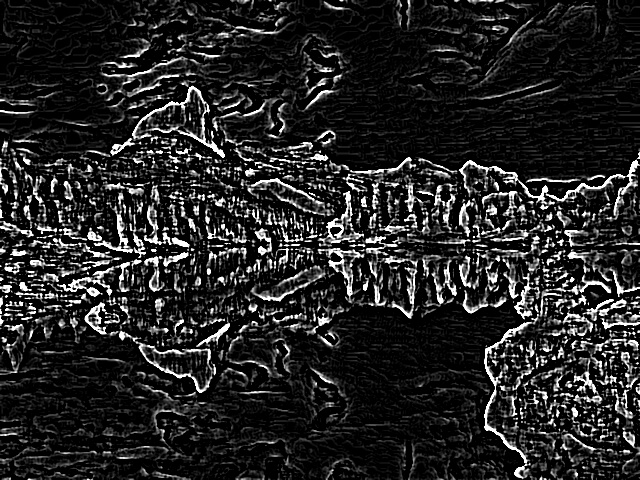
\epsfig{file=kepek/Cartoon1_laplacian.jpg,scale=0.45}
\caption{Laplace éldetektálás} 
\label{fig:2_cartoon3}
\end{figure}

\SubSection{Küszöbölés}

Az éldetektálás után, alkalmaztam egy küszöbölést amivel létrejött egy maszk, amit összeraktam az eredeti képpel (\ref{fig:2_cartoon4}. ábra).

\begin{figure}[h!]
\centering
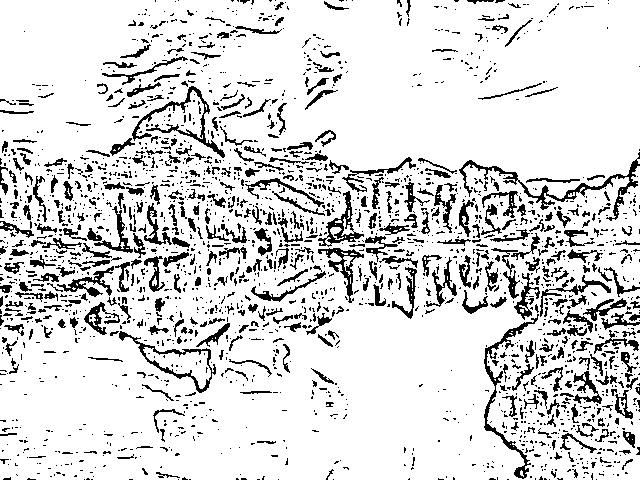
\epsfig{file=kepek/Cartoon1_thresh.jpg,scale=0.45}
\caption{Küszöbölés} 
\label{fig:2_cartoon4}
\end{figure}

Így készült el végeredményként a \textit{Cartoon filter}, melynek az eredménye \aref{fig:2_cartoon5}. ábrán látható.

\begin{figure}[h!]
\centering
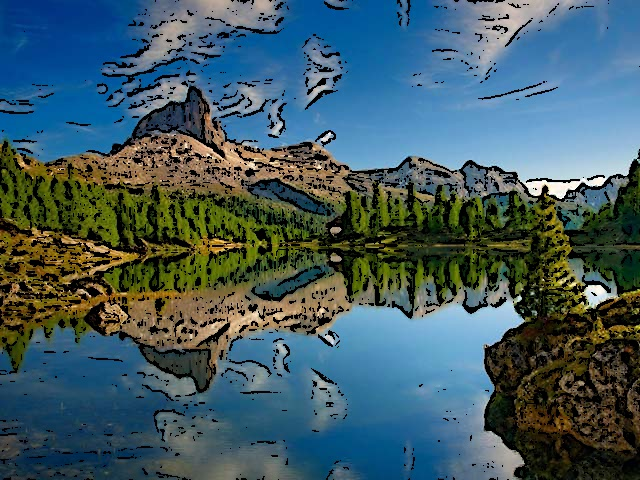
\epsfig{file=kepek/Cartoon1_filter1.jpg,scale=0.45}
\caption{Cartoon filter} 
\label{fig:2_cartoon5}
\end{figure}

\Section{Aquarelle-style filter}

Az utolsó saját szűrő amit készítettem az egy egyszerű vízfesték (\textit{aquarell}) hatású szűrő. Ez a szűrő teljesen más technikával készült mint az eddigiek. Nem használtam éldetektálást illetve küszöbölést sem. Az eredeti képpel dolgoztam végig, nem maszkoltam. A szűrés két lépésben megoldhatónak bizonyult. Elég egy átlagoló szűrés és egy mean shift szegmentálás egymást követően alkalmazni (\ref{fig:paint}. ábra).

\begin{figure}[h!]
\centering
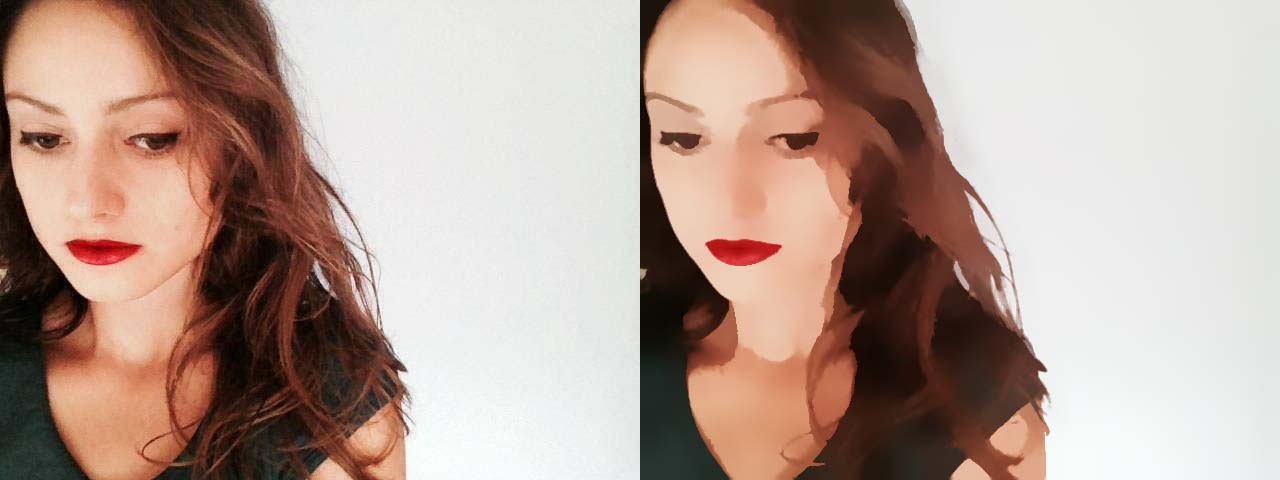
\epsfig{file=kepek/4_paint_filter.jpg,width=15cm, height=5.625cm}
\caption{Aquarelle-style filter (forrás: \textit{https://marieclaire.hu/kultura/2015/11/24/nem-mindig-az-a-cel-hogy-a-nezo-jol-erezze-magat-interju-kokai-tundevel/})} 
\label{fig:paint}
\end{figure}

\SubSection{Átlagoló szűrő}

Átlagoló szűrővel elmostam az eredeti színes képet, hogy az apróbb zajokat kiszűrjem (\ref{fig:paint1}. ábra).

\begin{figure}[h!]
\centering
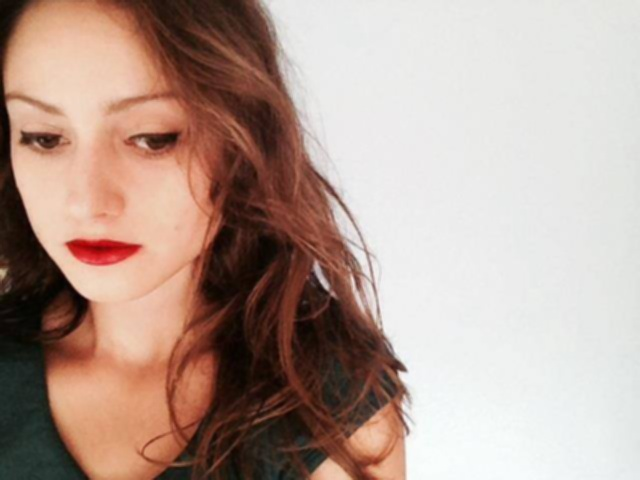
\epsfig{file=kepek/Paint_filter_blur.jpg,scale=0.48}
\caption{Átlagoló szűrő  } 
\label{fig:paint1}
\end{figure}

\SubSection{Mean shift szegmentálás}

Minden egyes adatpontnál a mean shift meghatároz egy ablakot, és kiszámítja az adatpont átlagát. Ezután az ablak közepét az átlag felé tolja, és megismétli az algoritmust, amíg konvergens. A mean shift egy nemparametrikus iteratív algoritmus vagy egy nemparametrikus sűrűségi gradiens becslés egy általánosított kernel megközelítés alkalmazásával (\ref{fig:paint2}. ábra).

\begin{figure}[h!]
\centering
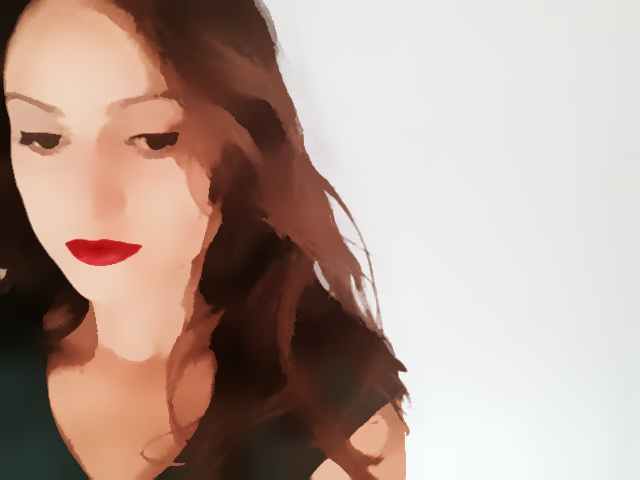
\epsfig{file=kepek/Paint_filter.jpg,scale=0.6}
\caption{Aquarelle-style filter, mean shift szegmentálás  eredménye} 
\label{fig:paint2}
\end{figure}

% https://gist.github.com/dgym/5532135
% Ide kellene felsorolni majd a saját szűrők algoritmusait!

\end{comment}